
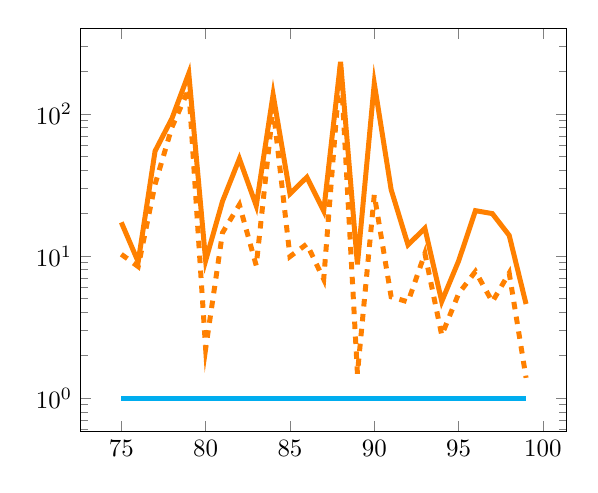
\begin{tikzpicture}[scale=0.9]
\begin{semilogyaxis}
\addplot[color=cyan,line width=2pt] coordinates {(75,1.0)(76,1.0)(77,1.0)(78,1.0)(79,1.0)(80,1.0)(81,1.0)(82,1.0)(83,1.0)(84,1.0)(85,1.0)(86,1.0)(87,1.0)(88,1.0)(89,1.0)(90,1.0)(91,1.0)(92,1.0)(93,1.0)(94,1.0)(95,1.0)(96,1.0)(97,1.0)(98,1.0)(99,1.0)};
\addplot[color=orange,line width=2pt] coordinates {(75,17.23448133228863)(76,9.091203623473808)(77,54.70371266251301)(78,92.82224877825617)(79,192.8140659082353)(80,9.278332542676328)(81,24.275659451809158)(82,48.3288729328444)(83,22.56924649575905)(84,136.868006906659)(85,27.393834930358008)(86,35.8335152284835)(87,20.73899414567274)(88,232.69665359894742)(89,8.71993382121161)(90,163.72732220101454)(91,29.276172633360165)(92,11.973363474999543)(93,15.657532425812946)(94,4.782696006201661)(95,9.215024439092637)(96,20.83920811328212)(97,19.86621933328564)(98,13.956461718678865)(99,4.589361414585358)};
\addplot[dashed,color=orange,line width=2pt] coordinates {(75,10.276394863687107)(76,8.419921491400814)(77,31.881607590333857)(78,80.53829541616251)(79,150.3035025411471)(80,2.2208956092748404)(81,14.582617621358004)(82,22.940802286247887)(83,8.560021647103632)(84,110.16307797044166)(85,9.903816116325455)(86,12.13431325064604)(87,6.848644594493099)(88,228.35410318196293)(89,1.4853039240605153)(90,26.933487288714513)(91,5.152652333730397)(92,4.748122858145427)(93,10.419080421557005)(94,2.7673575482137682)(95,5.4259035434750365)(96,7.780314339026608)(97,4.758487731099222)(98,7.5832900205981595)(99,1.3866364605136934)};

\end{semilogyaxis}
\end{tikzpicture}
